\documentclass[a4paper,twoside]{article}
\usepackage[T1]{fontenc}
\usepackage[bahasa]{babel}
\usepackage{graphicx}
\usepackage{graphics}
\usepackage{float}
\usepackage[cm]{fullpage}
\pagestyle{myheadings}
\usepackage{etoolbox}
\usepackage{setspace} 
\usepackage{lipsum} 
\setlength{\headsep}{30pt}
\usepackage[inner=2cm,outer=2.5cm,top=2.5cm,bottom=2cm]{geometry} %margin
% \pagestyle{empty}

\makeatletter
\renewcommand{\@maketitle} {\begin{center} {\LARGE \textbf{ \textsc{\@title}} \par} \bigskip {\large \textbf{\textsc{\@author}} }\end{center} }
\renewcommand{\thispagestyle}[1]{}
\markright{\textbf{\textsc{AIF184001/AIF184002 \textemdash Rencana Kerja Tugas Akhir \textemdash Sem. Ganjil 2023/2024}}}

\newcommand{\HRule}{\rule{\linewidth}{0.4mm}}
\renewcommand{\baselinestretch}{1}
\setlength{\parindent}{0 pt}
\setlength{\parskip}{6 pt}

\onehalfspacing
 
\begin{document}

\title{\@judultopik}
\author{\nama \textendash \@npm} 

%tulis nama dan NPM anda di sini:
\newcommand{\nama}{Andreas Ronaldi}
\newcommand{\@npm}{6182101026}
\newcommand{\@judultopik}{Pemutar Ulang Ketikan Mahasiswa pada SharIF Judge } % Judul/topik anda
\newcommand{\jumpemb}{1} % Jumlah pembimbing, 1 atau 2
\newcommand{\tanggal}{09/18/2024}

% Dokumen hasil template ini harus dicetak bolak-balik !!!!

\maketitle

\pagenumbering{arabic}

\section{Deskripsi}
Tugas merupakan sebuah alat bantu untuk menilai pemahaman mahasiswa yang diberikan oleh dosen. Salah satu tugas yang diberikan kepada mahasiswa informatika adalah tugas koding yang biasanya dinilai berdasarkan ketepatan keluaran dari sebuah masukkan yang sudah ditentukan sebelumnya. Tetapi melakukan penilaian kode merupakan sebuah hal yang sulit untuk dilakukan karena dibutuhkannya penilaian untuk setiap kode yang dikumpulkan mahasiswa. Maka dari itu website judge dibuat untuk memudahkan pekerjaan tersebut. Judge merupakan sebuah website yang akan menilai sebuah kode dengan menjalankannya berdasarkan masukkan yang ditentukan dan menyamakan keluaran dari kode dengan keluaran yang sudah ditetapkan oleh pembuat soal. 

Cara penilaian ini digunakan oleh Teknik Informatika UNPAR untuk menilai hasil kode dari para mahasiswanya. Judge yang digunakan adalah SharIF-Judge\footnote{https://github.com/ifunpar/SharIF-Judge} dimodifikasi oleh Stillmen Vallian terhadap Sharif-Judge\footnote{https://github.com/mjnaderi/Sharif-Judge} buatan Mohammad Javad Naderi dengan \textit{framework} CodeIgniter dan Bash. Berikut merupakan halaman utama setelah masuk ke dalam website SharIF-Judge.

\begin{figure}[H]
    \centering
    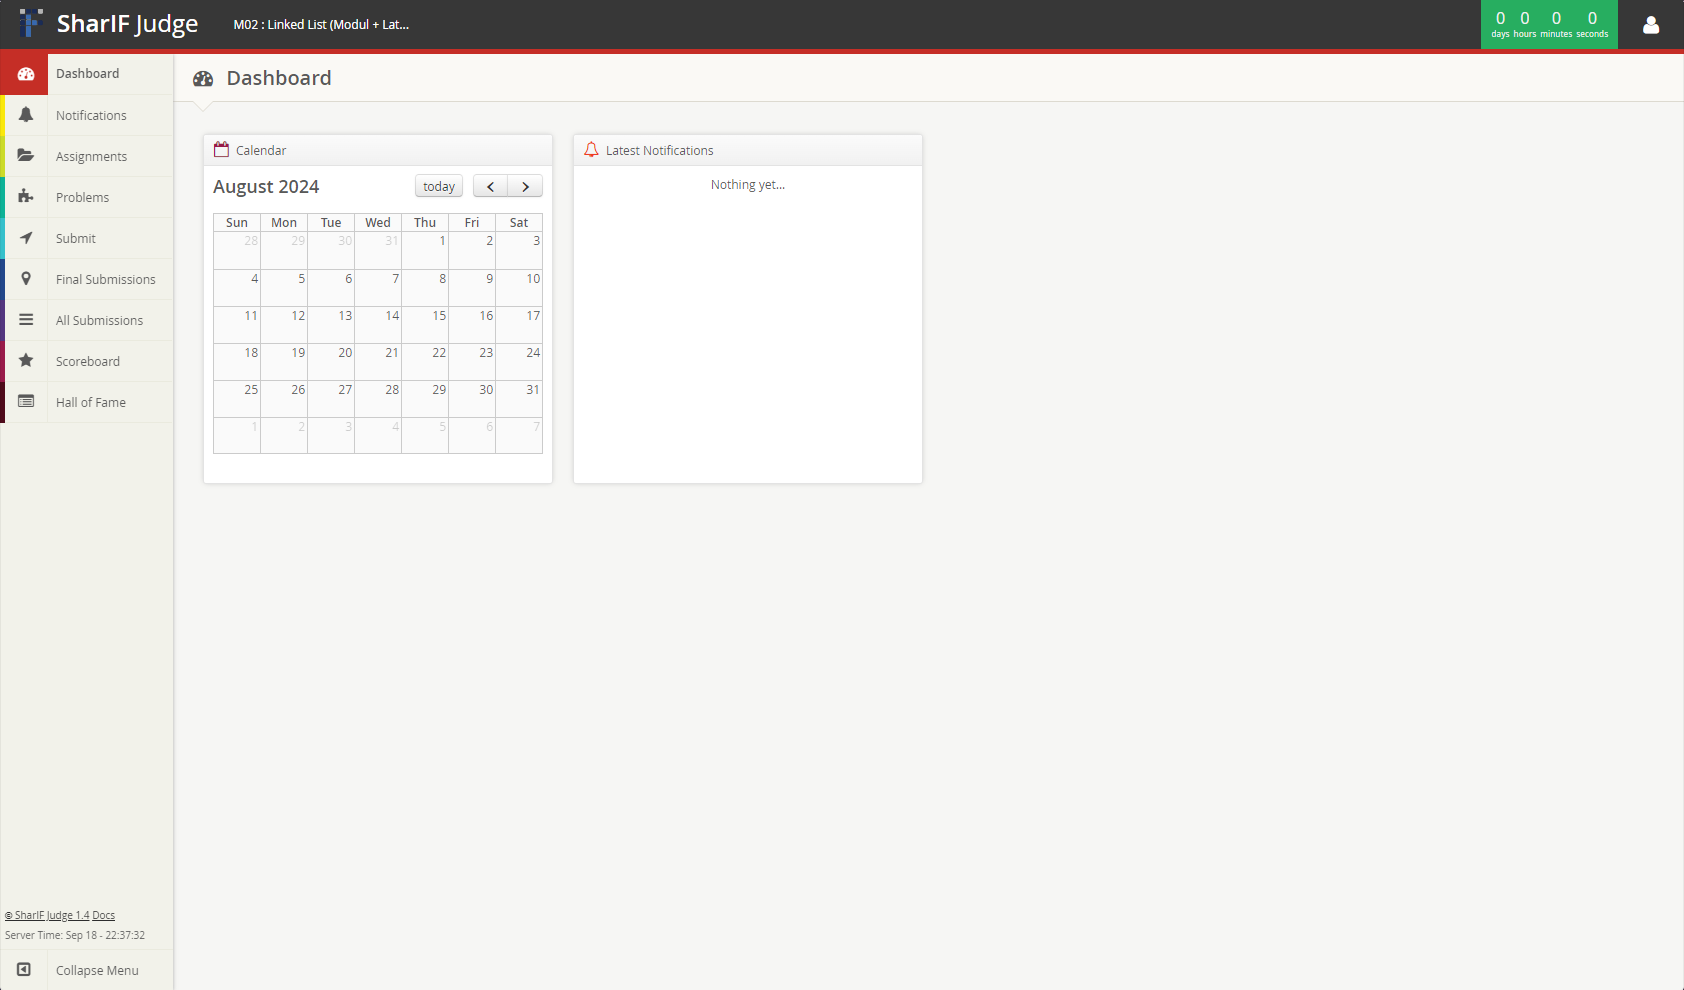
\includegraphics[width=0.75\linewidth]{dashboard.png}
    \caption{Tampilan awal SharIF-Judge}
\end{figure}

Tugas akhir ini merupakan sebuah pengembangan selanjutnya dari skripsi yang bertopik "Implementasi editor kode pada Sharif Judge"\footnote{Nicholas Aditya Halim, “Implementasi Editor Kode pada SharIF Judge”, 2021} oleh Nicholas Aditya Halim. Skripsi tersebut menceritakan bahwa judge ini tidak memiliki kemampuan untuk mengawasi proses pembuatan kode program karena para mahasiswa menggunakan aplikasi eksternal untuk pembuatan kode program tersebut. Sehingga dibuatnya modifikasi terhadap SharIF-Judge untuk menambahkan \textit{Intergrated Development Enviroment} (IDE), sebuah aplikasi untuk mengedit, mengompilasi, dan menjalankan kode program pada SharIF-Judge dengan editor kode bernama Ace\footnote{https://ace.c9.io/}. Berikut merupakan tampilan editor kode yang sudah diimplementasikan pada SharIF-Judge.

\begin{figure}[H]
    \centering
    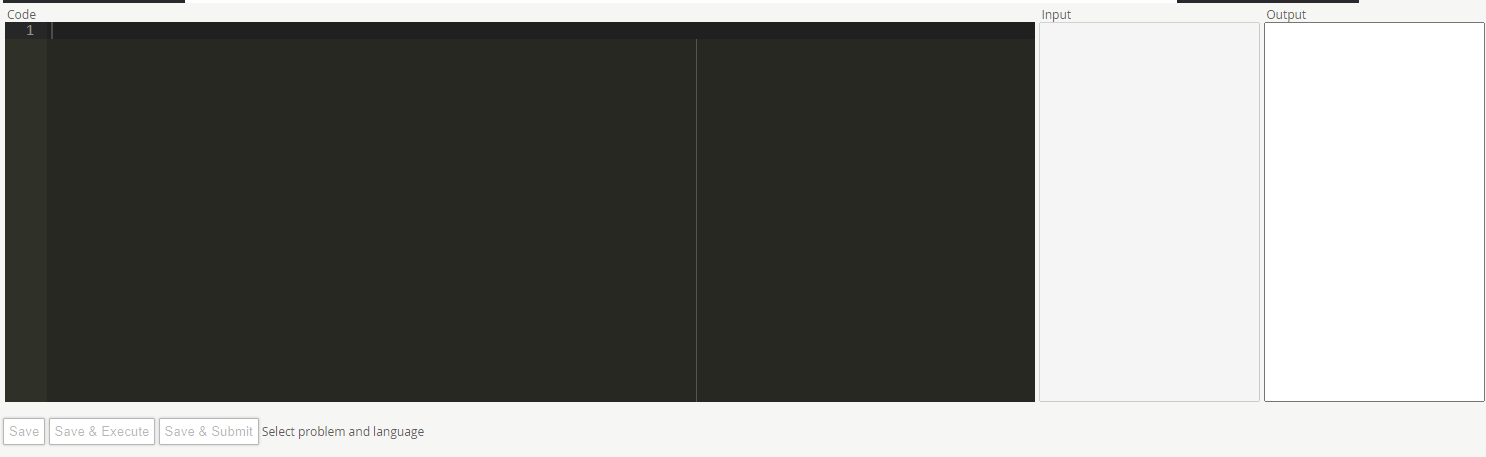
\includegraphics[width=0.75\linewidth]{kode-editor.png}
    \caption{Tampilan editor kode pada SharIF-Judge}
\end{figure}

Ace merupakan editor kode yang dibuat dengan bahasa pemograman \textit{JavaScript} dan merupakan salah satu editor kode yang dipakai oleh banyak website. Ace juga menyediakan ke stabilan dan kecepatan yang tinggi. Dengan mengunakannya editor kode Ace, SharIF-Judge memiliki banyak fitur bawaan yang mendukung editor kode pada umumnya seperti \textit{syntax highlighting} untuk semua bahasa pemrograman yang dipakai di teknik informatika UNPAR. Maka dari itu Ace dipilih sebagai editor kode yang dipakai untuk SharIF-Judge. Dengan Ace banyak fitur IDE yang dapat diimplementasikan yaitu mengedit kode dalam website secara langsung, meyimpan dan memuat kode untuk setiap permasalahan, dan menjalankan kode yang sudah di tuliskan pada IDE sesuai dengan input yang ditentukan mahasiswa. 

Pada tugas akhir ini, akan dibuat kode rekaman di IDE yang tersedia pada SharIF-Judge untuk membantu pengawasan dengan merekam dan memutar ulang ketikan di IDE. Tugas ini akan membuat pengawasan terhadap kegiatan kuliah lebih mudah untuk pengawas dan dapat menjadi bukti kecurangan jika dibutuhkan.

\section{Rumusan Masalah}
Rumusan Masalah yang akan dibahas pada tugas akhir ini adalah:
 \begin{enumerate}
     % \item Bagaimana agar editor kode lebih mudah untuk dipakai oleh mahasiswa.
     \item Bagaimana mengimplementasikan perekaman sistem untuk ketikan mahasiswa pada IDE SharIF-Judge?
     \item Bagaimana cara memperlihatkan pemutaran ulang ketikam kepada pengawas/dosen pada SharIF-Judge?
     \item Bagaimana cara menyimpan data pemutaran ulang mahasiswa secara rutin dengan otomatis dan tidak mengambil penyimpanan \textit{database} sangat besar?
 \end{enumerate}

\section{Tujuan}
Tujuan yang ingin dicapai skripsi ini adalah sebagai berikut:
    \begin{enumerate}
        % \item Mengimplementasikan kode editor mirip dengan aplikasi eksternal yang dipakai mahasiswa.
        \item Mengimplementasikan perekaman sistem untuk ketikan mahasiswa pada IDE SharIF-Judge.
        \item Mengimplementasikan sistem pemutaran ulang ketikan pada SharIF-Judge.
        \item Mencari cara peminmpanan data efektif dan mengimplementasikannya pada perekaman dan pemutaran ulang ketikan. 
    \end{enumerate}

\section{Deskripsi Perangkat Lunak}

Perangkat lunak akhir yang akan dibuat memiliki fitur minimal sebagai berikut:
\begin{itemize}
	\item SharIF-Judge dapat merekan semua event-event (ketikan, save, load, test) yang terjadi pada IDE.
    \item SharIF-Judge dapat menyimpan semua rekaman mahasiswa dengan tidak mengambil penyimpanan \textit{database} sangat besar.
    \item Dosen dapat menjalankan ulang rekaman ketikan mahasiswa yang terjadi pada IDE SharIF-Judge.

    % ide dari saya yang mungkin bisa membantu user baru lebih tertarik pakai IDE-nya
    % \item Pengguna dapat membuat kode editor di halaman baru
    % \item Pengguna dapat memilih problem langsung di kode editor-nya
    % \item Pengguna dapat merun beberapa input secara bersamaan
		
\end{itemize}

\section{Detail Pengerjaan Tugas Akhir}

Bagian-bagian pekerjaan skripsi ini adalah sebagai berikut :
	\begin{enumerate}

        \item Melakukan studi tentang PHP terutama \textit{framework} CodeIgniter dan editor kode Ace.
        \item Melakukan studi tentang cara penyimpanan rekaman ketikan
        \item Memodelkan dan merencanakan perubahan pada structur website dan database pada SharIF-Judge Unpar
        \item Mengimplementasikan rekaman ketikan pada SharIF-Judge
        \item Melakukan Pengujian dan eksperimen
        \item Menulis dokumen skripsi tugas akhir
 
	\end{enumerate}

\section{Rencana Kerja}
Rincian capaian yang direncanakan di Tugas Akhir 1 adalah sebagai berikut:
\begin{enumerate}
\item Mempelajari tentang PHP, \textit{framework} CodeIgniter, dan editor kode Ace
\item Melakukan studi tentang cara penyimpanan rekaman ketikan
\item Memodelkan dan merencanakan perubahan pada structur website dan database pada SharIF-Judge Unpar
\item Menulis sebagian dokumen tugas akhir yaitu bab 1, 2, 3
\end{enumerate}

Sedangkan yang akan diselesaikan di Tugas Akhir 2 adalah sebagai berikut:
\begin{enumerate}
\item Mengimplementasikan rekaman ketikan pada SharIF-Judge
\item Melakukan Pengujian dan eksperimen
\item Melanjutkan penulis dokumen tugas akhir yaitu bab 4, 5, 6 
\end{enumerate}

\vspace{1cm}
\centering Bandung, \tanggal\\
\vspace{2cm} \nama \\ 
\vspace{1cm}

Menyetujui, \\
\ifdefstring{\jumpemb}{2}{
\vspace{1.5cm}
\begin{centering} Menyetujui,\\ \end{centering} \vspace{0.75cm}
\begin{minipage}[b]{0.45\linewidth}
% \centering Bandung, \makebox[0.5cm]{\hrulefill}/\makebox[0.5cm]{\hrulefill}/2013 \\
\vspace{2cm} Nama: \makebox[3cm]{\hrulefill}\\ Pembimbing Utama
\end{minipage} \hspace{0.5cm}
\begin{minipage}[b]{0.45\linewidth}
% \centering Bandung, \makebox[0.5cm]{\hrulefill}/\makebox[0.5cm]{\hrulefill}/2013\\
\vspace{2cm} Nama: \makebox[3cm]{\hrulefill}\\ Pembimbing Pendamping
\end{minipage}
\vspace{0.5cm}
}{
% \centering Bandung, \makebox[0.5cm]{\hrulefill}/\makebox[0.5cm]{\hrulefill}/2013\\
\vspace{2cm} Nama: Pascal Alfadian Nugroho, S.Kom., M.Comp.\\ Pembimbing Tunggal
}
\end{document}
